% \section{Literature Survey}

% This chapter consists of two parts.  In part one, give any necessary engineering and non-engineering backgrounds that you see important for the complete understanding of your project. These backgrounds include, but are not limited to, facts, theory, formulas, algorithms and techniques. In other words, any pivotal knowledge to your project should be given, discussed, and properly defined. In part two give a short literature review of the latest publications related to your project within past three years if applicable.  Specially in this chapter, avoid lengthy unrelated discussion. More important, copy-and-paste should never be used. You have to write everything with your style and wording.

% In this space, before the first section, write an introductory paragraph to describe the topics and organization of the chapter

This chapter will enlight you with all the necessary background needed to fully comprehend the inner-workings of our separate modules, and the project as a whole.

To make it simple for our readers, we started this chapter with a very simple -yet important- non engineering section \ref{Personality Analysis} named \textit{Personality Analysis}; that plays an important role in understanding the prediction and classification of behavioural characteristics.\\

Then we follow with a full ride of our needed information in Machine Intelligence, starting from the pure definition of \textit{machine learning strategy} section \ref{Machine Learning Strategy}, the importance and the need of \textit{artificial neural networks} section \ref{Artificial Neural Network}, \textit{convolutional neural networks} and its major benefits when it comes to extracting features from images at section \ref{Convolutional Neural Network}, then we follow with \textit{sequence models} and its related subjects such as word2vec and embeddings at section \ref{Sequence Models}, and finish our journey with \textit{transfer learning} at section \ref{Transfer Learning}.\\

To fully comprehend main concepts used in distributed system we introduce two easily-clarified sections; \textit{CAP theorem} section \ref{sec:cap} to be familiar with terminology used later, and \textit{Load Balancing} section \ref{sec:Load} the main concept of our distributed system architecture.\\

Finally, we finish with comparative studies tackling the same problems we are facing section \ref{sec:comparitive}, and implementation approaches we decided to take at section \ref{sec:implemented}.

\section{Personality Analysis}
\label{Personality Analysis}
Scientist and psychologist defined models that describe human personality. The most popular models are \textbf{Big5/OCEAN} and  \textbf{Myers Briggs Type Indicator(MBTI)} models.

\subsection{Big5 personality model}
It divides personality into 5 spectrum \textbf{O}penness to experience, \textbf{C}onscientiousness, \textbf{E}Extroversion, \textbf{A}greeableness and \textbf{N}euroticism (\textbf{OCEAN}) or \textbf{Big5} where each spectrum defines a certain part of a person's personality.\cite{big5}\newline

\textbf{Openness to experience: }people who have high openness scores are curious about everything and eager to learn new experiences and things, they are more likely to be more adventurous and creative, while others who have low scores are more traditional and not very imaginative, they resist new ideas. [ Creative Vs Traditional ]\newline

\textbf{Conscientiousness: }people who have high Conscientiousness scores tend to be more organized, efficient and mindful, they plan things ahead with its consequences, while others who have low scores are more careless, don’t like scheduling nor taking care of things. [ Organized Vs Careless ] \newline

\textbf{Extroversion: }people who have high extroversion scores are outgoing and more likely to gain energy and excitement around other people, they like to talk and easily make friends, while others who have low scores are more reserved and feel drained from socializing, they dislike talking and find difficulty in it . [ Social Vs Reserved ]\newline

\textbf{Agreeableness: }people who have high agreeableness scores tend to be more cooperative, care about others, help and assist others who are in need of help, while others who have low scores tend to be more competitive, have a little interest in others and their problems. [ Cooperative Vs Competitive ]\newline

\textbf{Neuroticism: } people who have high neuroticism scores tend to have more mood swing, anxiety and their feelings are easily affected, while others who have low scores tend to be more calm, relaxed and emotionally stable [ Sensitive Vs Calm ]\newline



\begin{figure}[h]
\centering
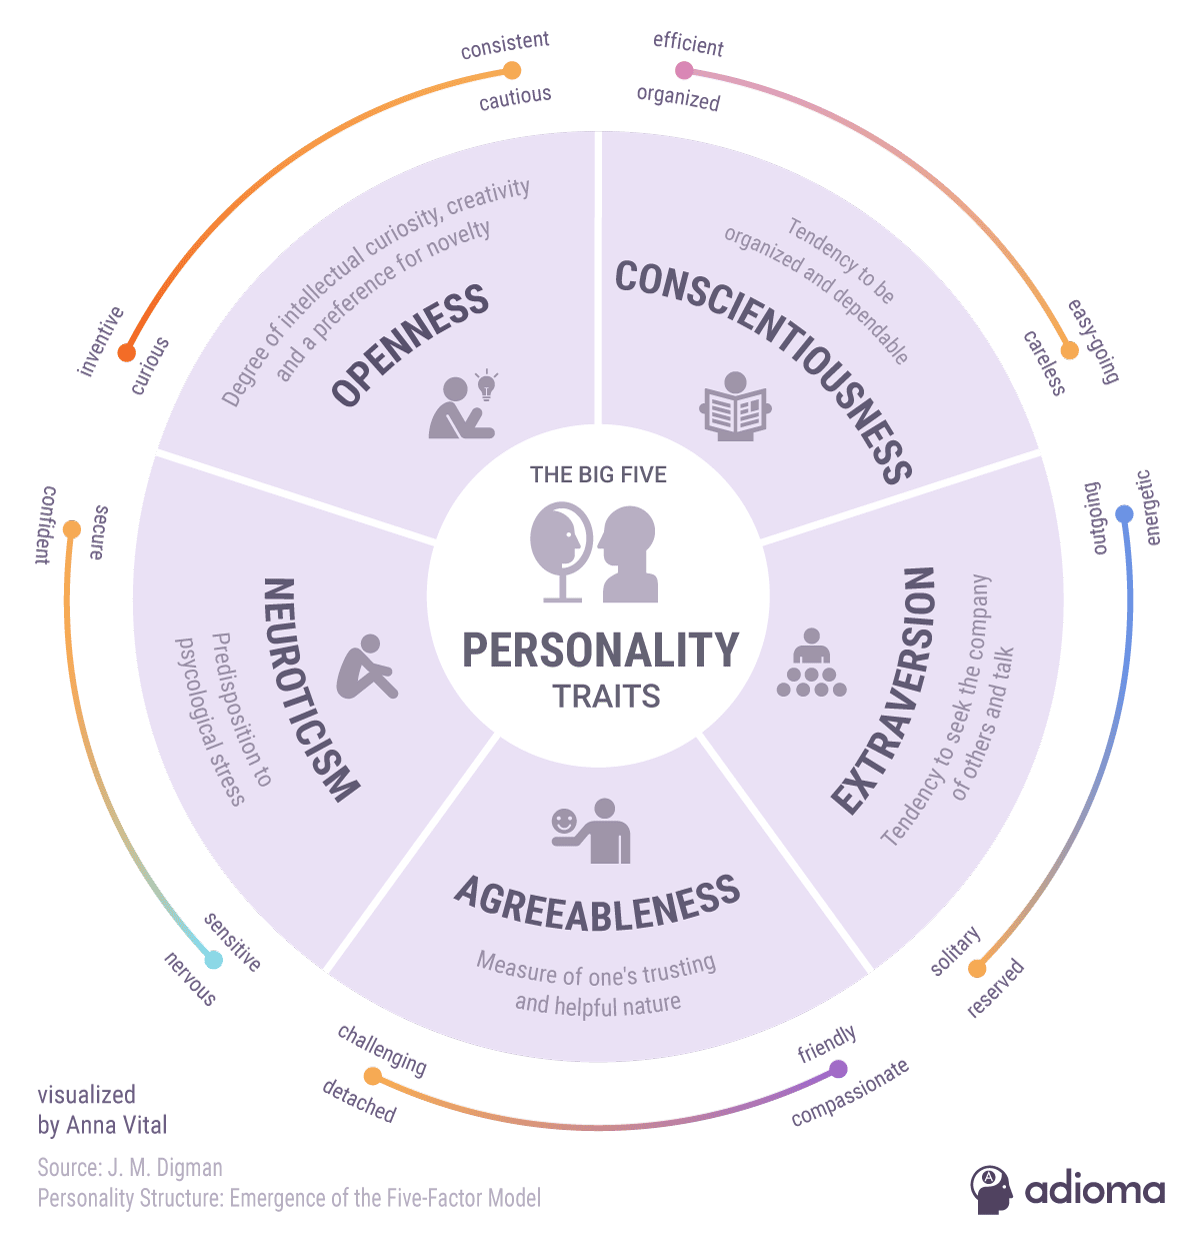
\includegraphics[width=15cm,height=15cm]{images/big5.png}
\caption{Big5 Spectrum \href{https://blog.adioma.com/wp-content/uploads/2018/11/big-five-personality-traits-infographic.png}{(\underline{source})}}
% \label{General model of ANN}
\end{figure}

\subsection{Myers-Briggs Type Personality Model(MBTI)}
\label{sec:mbti_ls}
MBTI is another model that defines human personality by looking into other perspectives. It consists of:
\begin{itemize}
  \item Extroverts(E) - Introverts(I)
  \item Sensors(S) - Intuitives(N)
  \item Thinkers(T) - Feelers(F)
  \item Judgers(J) - Perceivers(P)
\end{itemize}


\textbf{Extroverts(E) - Introverts(I): }Extroverts are energized people who enjoy communicating and making friends, while Introverts who prefer to work alone.\newline

\textbf{Sensors(S) - Intuitives(N): }Sensors are people who like to focus on details and apply past experience to come up with solutions to problems, while Intuitives focus on big pictures and seek creativity to come up with solutions.\newline

\textbf{Thinkers(T) - Feelers(F): }Thinkers are people who tend to make decisions based on logical analysis, while Feelers are people who tend to decide based on their own personal feelings.\newline

\textbf{Judgers(J) - Perceivers(P): }Judgers are people who tend to make and stick to their plan, while  Perceivers are people who tend to be more flexible with plans.\newline

By combining the above 4 categories we form a certain personality (eg. ISTJ), each has its own intuition, so we get 16 possible personalities \cite{MBTI}.

There are multiple conventions and different variations. Figure \ref{fig:mbti_ls_1} show these variations. Such a diverse combination of traits (personalities) span the the spectrum of different personalities. For example, "The Architect" is able to work in positions where designs are required, and "The Adventurer" may be productive in marketing field ..etc.



\begin{figure}[h]
\centering
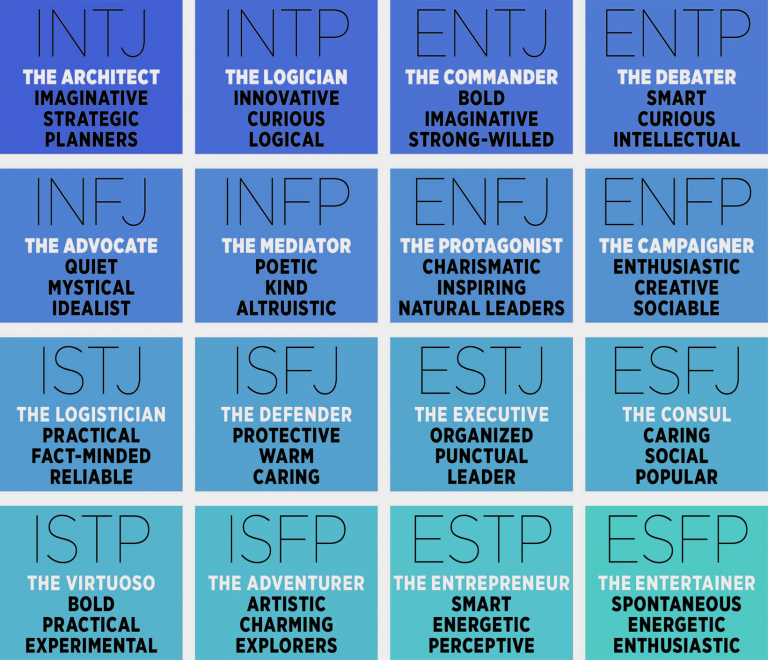
\includegraphics[width=0.6\textwidth]{images/MBTI.png}
\caption{Different Combinations of MBTI \href{https://practicalpie.com/wp-content/uploads/2021/03/Printable-Myers-Briggs-Matrix-768x660.png}{(\underline{source})}}
\label{fig:mbti_ls_1}
\end{figure}


% \begin{figure}[ht]
% \centering
% \begin{minipage}[b]{0.45\linewidth}
% 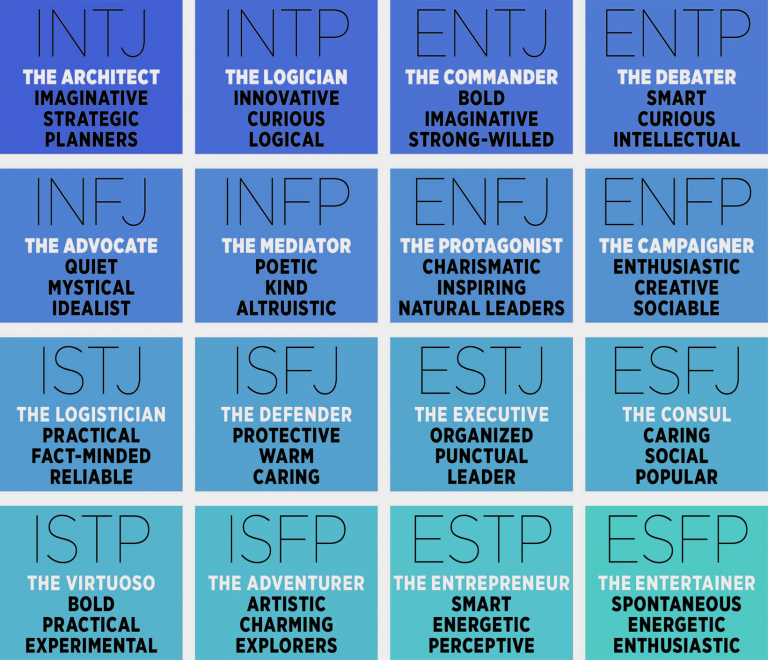
\includegraphics[scale=0.4]{images/MBTI.png}
% \caption{}
% \label{fig:mbti_ls_1}
% \end{minipage}
% \quad
% \begin{minipage}[b]{0.45\linewidth}
% 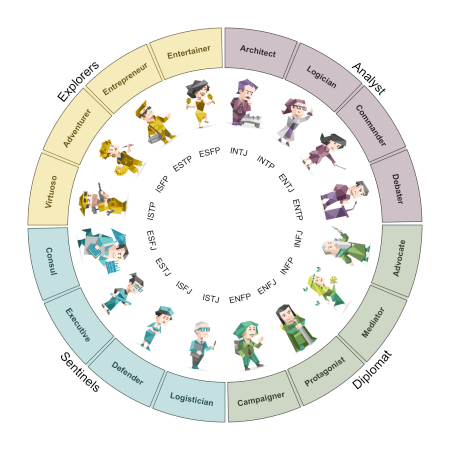
\includegraphics[scale=0.55]{images/MBTI_cartoon.png}
% \caption{MBTI Spectrum \href{https://www.pinterest.com/pin/587227238903993347/}{(\underline{source})}}
% \label{fig:mbti_ls_2}
% \end{minipage}
% \end{figure}


\pagebreak

\section{Machine Learning Strategy}
\label{Machine Learning Strategy}
Machine Learning is a subarea of artificial intelligence, where machines learn to do a certain task based on previous experience (dataset). Many steps are required to build a statistical model that is able to achieve the best outcome possible.

We introduce this section to illustrate important building steps of any artificial intelligence system. These steps are:

\begin{itemize}
  \item Dataset acquisition
  \item Data pre-processing/preparation
  \item Features extraction
  \item Model training
  \item Model evaluation
  \item Parameters tuning
  \item Making predictions
\end{itemize}

\textbf{Dataset acquisition:}Data mostly collected from different sources from the internet in different forms/formats, this step decides how accurate the model will be based on the quality and quantity of the dataset.
Data can be in three main forms , \textit{structured}, often stored in tabular forms, \textit{unstructured}, like images and text, and \textit{semi-structured}, like json and xml files.\newline

\textbf{Data pre-processing/preparation: }Data collected from internet, by experiments, or collected manually are noisy and not ready to be processed right away; that is why we need to prepare it to be correctly processed. This includes:
\begin{itemize}
  \item Cleaning; ( remove duplicates, deal with missing records, correct errors, normalization,....).
  \item Visualizing; to detect relationships and patterns.
  \item Randomizing; to remove order effect.
  \item Splitting; into train/validation/test sets.
  \item Transforming; to focus on information rather than data. \newline
\end{itemize} 

\textbf{Features extraction: }Selecting or extracting features that need to be learnt/processed. Either by selecting some of them, or by transforming. This process needs engineering and thinking.\newline

\textbf{Model training: }Building the model is the most intuitive step of them all, it consists of numerous trials and evaluation checks. The main goal is trying to make predictions of the best outcome based on fed data. This step requires a lot of resources(time, computation, suitable amount of data) for the model to train.\newline

\textbf{Model evaluation: }Test the model on data different from that used during training, which is meant to be somewhat representative of the model performance and this includes using some metrics to measure the model performance.\newline

\textbf{Parameters tuning: }This refers to both parameters and hyper-parameters tuning, which could be the number of training steps, learning rate and initialization values; this step is very important for improving model performance.\newline

\textbf{Making predictions: }Deploying the machine to do the task it was trained for, using further tests.\newline

We have adopted these techniques in all steps of our project.

\pagebreak

\section{Artificial Neural Network}
\label{Artificial Neural Network}
Artificial neural network, or multi-layer perceptron, is at the very core and considered the main asset of deep learning. ANN are usually composed of \textit{input layer}, the set of independent variables/features, \textit{output layer}, that represents the final predicted output, \textit{hidden layer(s)}, which consist of neurons where outputs from the previous layer are transformed so next layer can make use of it, and \textit{activation functions} simple functions that exploit their nature to propose non-linearity into the ANN.

They can be used for two main prediction aspects: 1- linear regression, where we aspire to predict a continuous value that best matches the input features, 2- classification, where categorical values are predicted.

We introduce this section; because in all of our three intelligent agents we used ANN for \textit{classification} of the final output, though it could be used for features extraction, but we used more complex architectures for that, such as (CNN and LSTM); so our main focus in this discussion will be predicting the best class that fits the input features.


\subsection{Architecture}
In the following section we define the architecture of ANN, and preview how a one simple neuron acts in the network.

\begin{figure}[h]
\centering
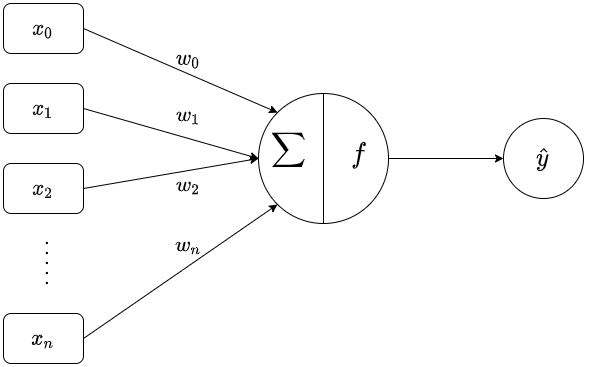
\includegraphics[width=0.6\textwidth]{images/ann_1.png}
\caption{General model of ANN}
\label{General model of ANN}
\end{figure}

For the above general model of ANN figure \ref{General model of ANN}, $\underset{1\times n}{\mathrm{X}}$ represents input features vector for one example, $\underset{n\times 1}{\mathrm{W}}$ is the weights matrix, summed, and then $f$ activation function is applied, producing $\hat{y}$, the predicted output for only one example. 

\begin{equation} \label{eq:general model of ann}
\hat{y} = f \left( \sum_{i=0}^{n} x_i w_i \right)
\end{equation}
\myequations{Neuron Function}

Though $X$ and $W$ should be represented as vectors here, but this should be applied for each example, so we denote them as matrices.

This linear summation is the main computation that occurs at each neuron of the network, stacking neurons vertically we produce layers, stacking layers horizontally, we produce network, in figure \ref{common arch of ann} we view the common architecture of ANN. Complex architectures composed of multiple layers with many neurons that should be able to extract very complex features, however, simpler architecture are usually favored.


\begin{figure}[h]
\centering
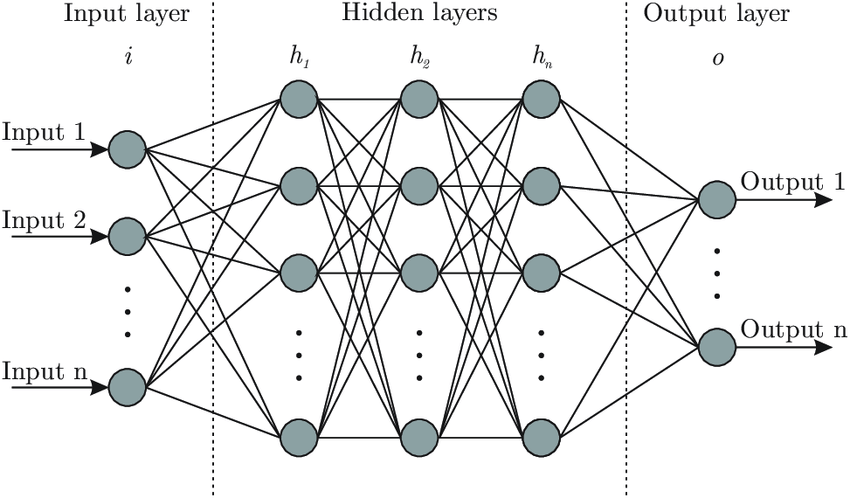
\includegraphics[width=0.8\textwidth]{images/neural_network.png}
\caption{Common architecture of ANN \href{https://www.researchgate.net/figure/Artificial-neural-network-architecture-ANN-i-h-1-h-2-h-n-o_fig1_321259051}{(\underline{source})}}
\label{common arch of ann}
\end{figure}

\subsection{Activation function}
\label{sec:activation_function}

An activation function, is a function that defines how the input weights values are transferred into output values. That is why it is called transfer function. Transformation may be done by applying one of different non-linear functions such as:
\begin{itemize}
  \item Sigmoid
  \item Rectified linear activation (ReLU)
  \item Hyperbolic tangent (Tanh)
  \item Leaky ReLU
  \item Maxout \newline
\end{itemize} 

We will discuss some of these functions that will be implemented later on in each of the agents. \newline

\textbf{1- ReLU: }It computes the function: $f(u)=max(0,u)$, the activation is thresholded at zero, see figure \ref{ReLU activation function}. One of the benefits of using ReLU is that it was found to greatly accelerate the convergence of stochastic gradient descent (explained at \ref{updating_weights}) compared to the sigmoid/tanh functions \cite{relu_cite}.\newline


\begin{figure}
    % \centering
    \begin{subfigure}[b]{0.5\textwidth}
        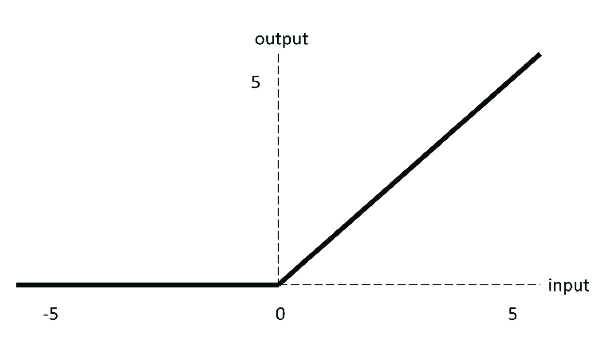
\includegraphics[width=7cm,height=5cm]{images/relu.png}
        \caption{ReLU activation function \href{https://www.researchgate.net/figure/ReLU-activation-function_fig7_333411007}{(\underline{source})}}
        \label{ReLU activation function}
    \end{subfigure}
    \hfill
    \begin{subfigure}[b]{0.5\textwidth}
        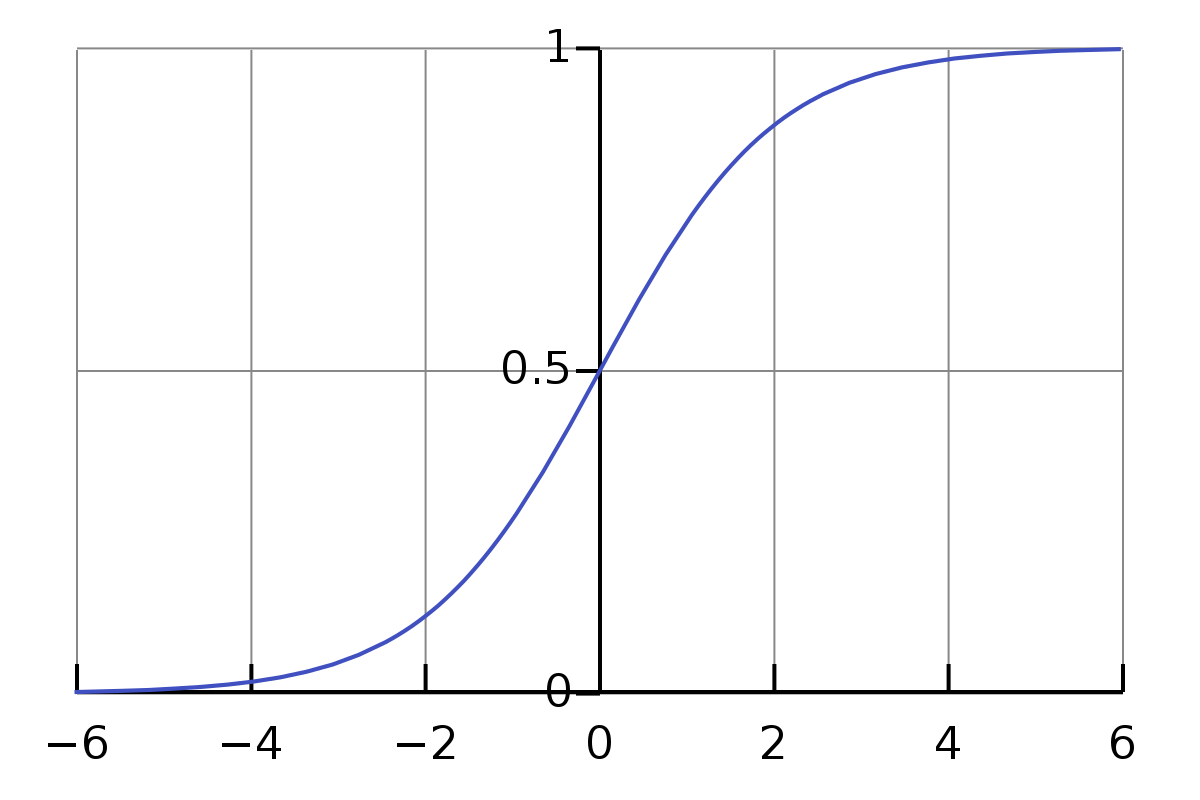
\includegraphics[width=7cm,height=5cm]{images/sigmoid.png}
        \caption{Sigmoid activation function \href{https://en.wikipedia.org/wiki/Sigmoid_function}{(\underline{source})}}
        \label{sigmoid_figure}
    \end{subfigure}
    \caption{Activation functions}
    \label{fig:activation functions}
\end{figure}

\textbf{2- Sigmoid} The sigmoid non-linearity has the mathematical form  $\sigma (x) = 1/(1 +  e^{-x})$ shown in figure \ref{sigmoid_figure}. Although its computations is relatively more expensive, but still used in sequence models (LSTM and GRU); due to its differential property that eases the computations through the network as a whole.


\subsection{Loss function}
\label{sec:loss function}
In order to evaluate our hypothesis (values of weights) we need a mathematical metric that represents the loss we suffer. Various loss functions are used depending on the application and the type of prediction desired (classification / regression), examples:

\begin{itemize}
    \item Cross-entropy loss
    \item Hinge loss
    \item Mean square error
\end{itemize}

We used ANN for classification within the three agents, cross-entropy function is more meaningful for this type of predictions.\newline

\textbf{Cross-entropy loss}, or log loss, measures the performance of a classification model whose output is a probability value between 0 and 1. Cross-entropy loss increases as the predicted probability diverges from the actual label. So, predicting a probability of .012 when the actual observation label is 1 would be bad and result in a high loss value relative to the other outcomes.

Figure \ref{cross_entropy} shows the range of possible loss values given a true observation. As the predicted probability $p$ approaches 1, log loss slowly decreases. As the predicted probability decreases, however, the log loss increases rapidly. Log loss penalizes both types of errors, but especially those predictions that are confident and wrong, formula for binary classification:
\begin{equation} \label{eq:cross_entropy}
L = - \left( (y \log {p}) + ( (1-y)\log{(1-p)} )  \right)
\end{equation}
\myequations{Cross-entropy binary}

For K classes:
\begin{equation}\label{eq:cross_entropy_2}
L = - \left(  \sum_{c=1}^{K} y_{i,c} \log {(p_{i,c})}  \right)
\end{equation}
\myequations{Cross-entropy multi-class}



Notice that $p$ is the prediction of class $i$ -assuming binary classification-, its value is in range of $[0,1]$, so if result is true $y=1$ then loss depends only on the left term, where the farther $p$ from $1$, the larger $L$ and vice versa.

\begin{figure}[h]
    \centering
    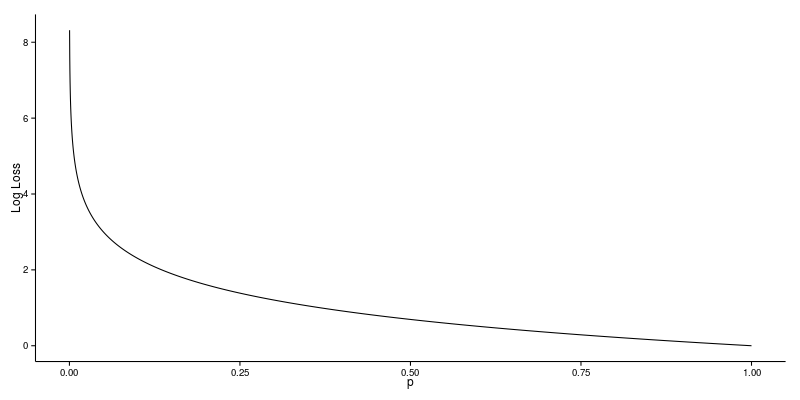
\includegraphics[width=7cm,height=5cm]{images/cross_entropy.png}
    \caption{Log loss when true label = 1 \href{https://ml-cheatsheet.readthedocs.io/en/latest/loss_functions.html}{(\underline{source})}}
    \label{cross_entropy}
\end{figure}

\subsection{Regularization}
\label{regularization}
Complex architectures tend to over-fit the dataset, leaving our model with the inability to accurately predict unseen examples, regularization is the concept of reducing over-fitting, and making the model more generalized, many techniques can be applied, such as:
\begin{itemize}
  \item Dropout
  \item L1 or L2
  \item Reducing model's complexity.
\end{itemize} 

\textbf{Dropout: }It’s a simple technique to prevent over-fitting, by simply dropping out some neurons from the network, this happens by randomly shutting off some neurons from learning. This improves generalizing to new data; because neurons are shut down in non-deterministic manner.\newline

\textbf{L2: }It's used to penalize complex architectures, we can quantify complexity using the L2 regularization formula, which defines the regularization term as the sum of the squares of all the feature weights:

\begin{equation} \label{eq:l2_reg}
    L2\; regularization\; term = \Vert W \Vert_2^2 = w_1^2 + w_2^2 +  ... + w_l^2
\end{equation}
\myequations{L2 regularization}


\subsection{Forward propagation}
To fully comprehend the life-cycle of updating ANN models, and how they learn and evolve, let us consider a simple example with one input layer, two hidden layers, and one output layer, that predicts binary classification value (ie. 0 or 1), like most of our cases in this project -except for the output dimensions of course-, see figure \ref{fig:main_example} for illustration.\newline

\begin{figure}
    \centering
    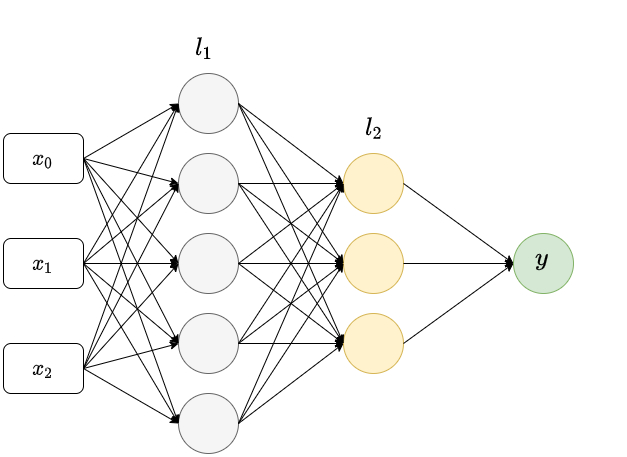
\includegraphics[width=0.8\textwidth]{images/ann_2.png}
    \caption{Main ANN example}
    \label{fig:main_example}
\end{figure}

Let us assume parameters and dimensions of this network:
\begin{itemize} 
    \item $M$ examples are processed, each having 3 features, hence dimension of $[X]$ is $\underset{5\times 3}{\mathrm{X}}$
    \item Two hidden layers $l_1$ and $l_2$, with 5 and 3 neurons respectively, hence number of layers $L = 3$.
    \item Three weights matrices are needed $\underset{3\times 5}{\mathrm{W^{[1]}}}$ , $\underset{5\times 3}{\mathrm{W^{[2]}}}$, and $\underset{3\times 1}{\mathrm{W^{[3]}}}$.
    \item ReLU activation function $f$.
    \item Binary classification, labels are 0 or 1.
    \item Cross-entropy loss metric.
    \item Softmax function applied at the last layer, will discuss it later.
\end{itemize}

Forward propagation is computing the prediction of $y$ which is $\hat{y}$, the resulting value from propagating example $i$ through the network, follow these equations for more illustration:

\begin{equation} \label{eq:forward_prop_1}
\begin{split}
    a^{[1]} = f \left( X \times W^{[1]} \right) \\
    a^{[2]} = f \left( a^{[1]} \times W^{[2]} \right) \\
    a^{[3]} = f \left( a^{[2]} \times W^{[3]} \right)
\end{split}
\end{equation}
\myequations{Forward propagation of three layers}


Notice that, $a^{[1]}$ are the grey cells, $a^{[2]}$ are the orange ones, and $a^{[3]}=\hat{y}$ is the green one. Also, the last hidden layer $l_2$ should not use ReLU activation function, instead it uses softmax function, to make normalized prediction of all of the outcomes that are present in the model.\newline

In general, denoting $X$ as $a^{[0]}$ and $a^{[l]}$ as $\hat{y}$:
\begin{equation}\label{eq:forward_prop_2}
    a^{[l]} = f \left( a^{[l-1]} \times W^{[l]} \right)
\end{equation}
\myequations{Forward propagation of L layers}

As we previously mentioned, we need to transform results from the final layer so that they are contained within the range of $[0,1]$, and also to be accurately representative of the accuracy predicted of each class, so we need to normalize output values using \textit{softmax} function.\newline

\begin{equation}\label{eq:softmax}
   \sigma (\hat{y_i}) = \frac{e^{\hat{y_i}}}{\sum_{j=1}^{K} e^{\hat{y_j}}}
\end{equation}
\myequations{Softmax function}


After that we compute the loss we suffered from this path, using cross-entropy loss \ref{eq:cross_entropy}.

See figure \ref{fig:forward_prop_3} for full vision view with a computation graph.

\begin{figure}
    \centering
    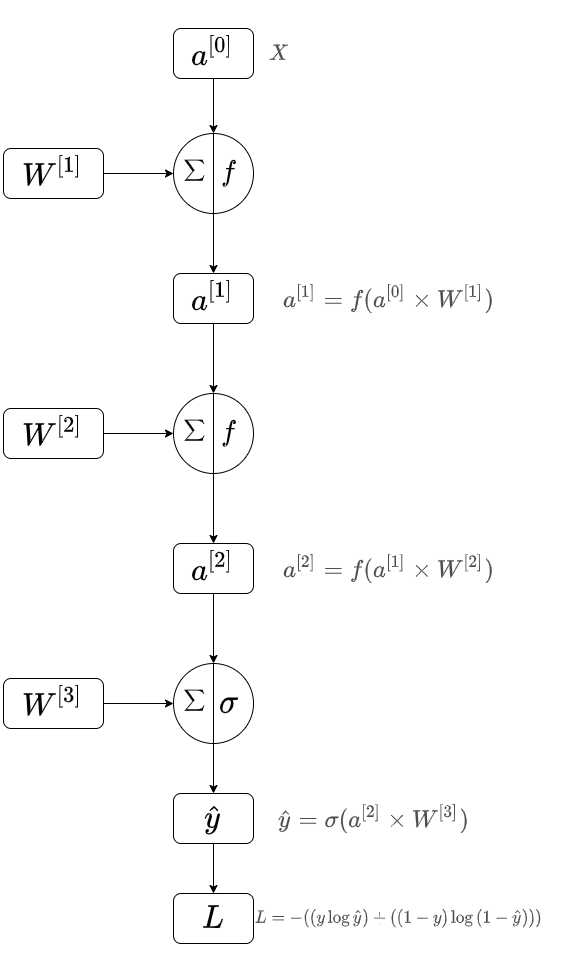
\includegraphics[width=0.9\textwidth]{images/forward_prop_3.png}
    \caption{Forward propagation}
    \label{fig:forward_prop_3}
\end{figure}

\subsection{Backward propagation}
Now that we have computed the loss due to our current hypothesis (weights), we need to figure out a way to optimize them. Optimization is a hill climbing process, where we aspire to reach global minimum of the loss (ie. minimizing the loss as much as possible), without getting stuck in a local minimum, or even worse, maximizing the loss to infinity.

Thus our goal becomes clearer now, we need to find the set of weights $Ws$ such that they produce the minimum value of $L$, see figure \ref{fig:global_minima}.

\begin{figure}[h]
\centering
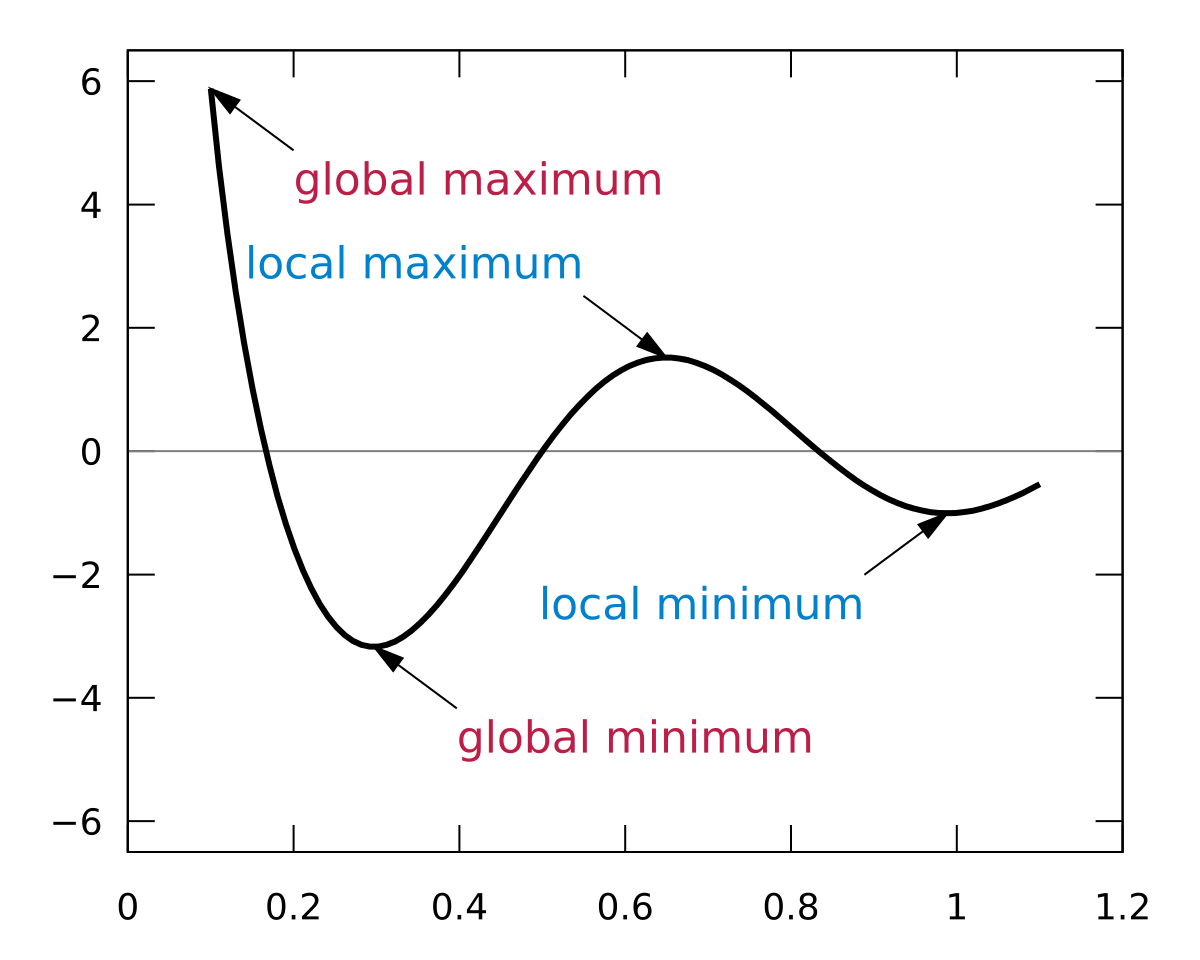
\includegraphics[width=0.6\textwidth]{images/global_minima.png}
\caption{Local/Global minimum \href{https://en.wikipedia.org/wiki/Maxima_and_minima}{(\underline{source})}}
\label{fig:global_minima}
\end{figure}

Earliest techniques used random guessing to find the best set of weights that fit the model, but when the space of weights becomes larger, in order of hundreds of millions, we can't rely on guessing for sure, that's why we needed statistical methods to come up with an update that guides the weights into finding global minimum for the loss function; differential equations come in handy, we need to find how much do the weights deviates from the optimal value (ie. $L=0$). By calculating the partial derivatives of $L$ -the loss function- with respect to each $W$ -weight variable- in the network, thus come up with an update value that if taken away from the current $W$, with a limiting value (learning rate $\alpha$) we believe that $L$ will reach fewer values, this is the popular \textit{gradient descent} algorithm.

The update rule looks like this:

\begin{equation} \label{eq:backward_prop_1}
    W^{[L]} = W^{[L]} - \alpha \frac{\partial L}{\partial W^{[L]}}
\end{equation}
\myequations{Gradient descent update rule}

Here $\alpha$ is known as the learning rate of the network, because it decides how big updates we perform, in other words, it tells us how big steps are we taking in the direction of the local minimum, i.e. what is the rate at which we are learning.

From the computation graph fig \ref{fig:forward_prop_3}, we can make a few observations which will help us calculate the partial derivatives. $L$ is a function of $a^{[3]}$, $a^{[3]}$ is in turn a function of $w^{[3]}$ and $a^{[2]}$, so to calculate the partial derivative of $L$ wrt. $w^{[3]}$ we will use the chain rule.

This gives us:

\begin{equation} \label{eq:backward_prop_2}
\begin{split}
    \frac{\partial L}{\partial W^{[3]}} &=  \frac{\partial L}{\partial a^{[3]}} \times \frac{\partial a^{[3]}}{\partial W^{[3]}}\\
    \frac{\partial L}{\partial W^{[2]}} &=  \frac{\partial L}{\partial a^{[3]}} \times \frac{\partial a^{[3]}}{\partial a^{[2]}} \times \frac{\partial a^{[2]}}{\partial W^{[2]}}\\
    \frac{\partial L}{\partial W^{[1]}} &=  \frac{\partial L}{\partial a^{[3]}} \times \frac{\partial a^{[3]}}{\partial a^{[2]}} \times \frac{\partial a^{[2]}}{\partial a^{[1]}} \times \frac{\partial a^{[1]}}{\partial W^{[1]}}
\end{split}
\end{equation}
\myequations{Backward partial derivatives}

This can be better understood from the computational figure \ref{fig:backward_prop_1}:

\begin{figure}
    \centering
    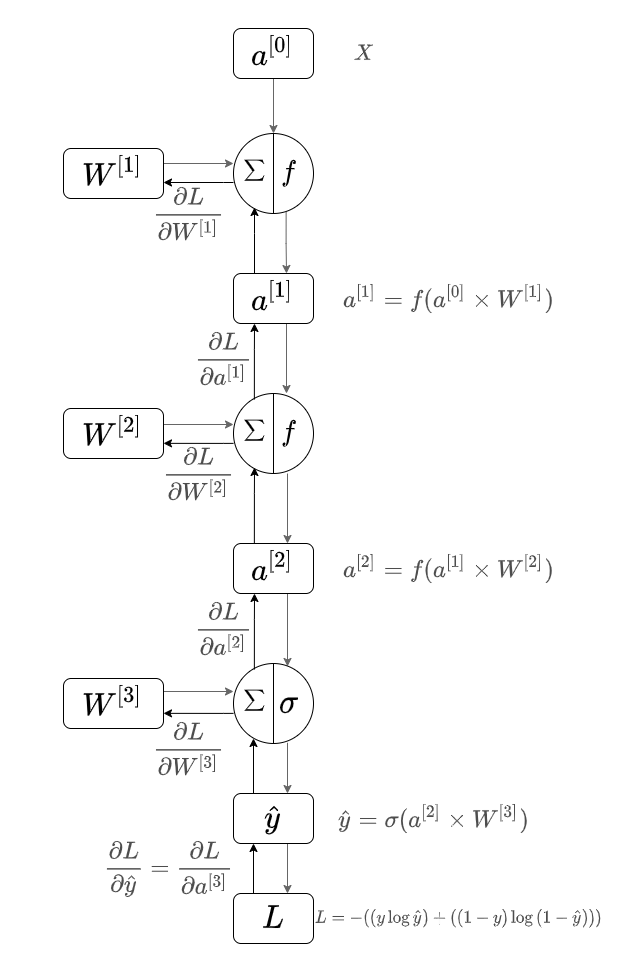
\includegraphics[width=0.9\textwidth]{images/backward_prop_1.png}
    \caption{Backward propagation}
    \label{fig:backward_prop_1}
\end{figure}



Calculations required for each of these steps equation: \ref{eq:backward_prop_2} depends on the used activation function, the partial derivative of ReLU function is:

\begin{equation} \label{eq:backward_prop_3}
    % \[
    f'(x)= 
\begin{cases}
    1,& \text{if } x\geq 0\\
    0,& \text{otherwise}
\end{cases}
% \]
\end{equation}
\myequations{Partial derivative of ReLU function}

Partial derivative of Sigmoid function is:

\begin{equation} \label{eq:backward_prop_4}
    f'(x)= f(x) \times (1 - f(x)) 
\end{equation}
\myequations{Partial derivative of Sigmoid function}

The value we choose for the learning rate $\alpha$ is going to require some testing. The learning rate is another one of those hyperparameters that we have to test and tune with each model before we know exactly where we want to set it, but as mentioned earlier, a typical guideline is to set it somewhere between 0.01 and 0.0001.

When setting the learning rate to a number on the higher side of this range, we risk the possibility of overshooting. This occurs when we take a step that's too large in the direction of the minimized loss function and shoot past this minimum and miss it.

To avoid this, we can set the learning rate to a number on the lower side of this range. With this option, since our steps will be really small, it will take us a lot longer to reach the point of minimized loss.
Overall, the act of choosing between a higher learning rate and a lower learning rate leaves us with this kind of trade-off idea.

\subsection{Updating weights} \label{updating_weights}
Finally, we come to a solid ground where we are able to update our hypothesis with new values that will guide the model towards global minimum. Simple updates are not that efficient, so various options exist for efficiently updating weights:

\begin{itemize}
    \item Stochastic gradient descent
    \item Momentum update
    \item Nesterov Momentum
    \item Adagrad
    \item RMSprop
    \item Adam
\end{itemize}

Through out our models we used Adam \cite{adam} optimization algorithm instead of the classical stochastic gradient descent procedure to update network weights iterative based in training data. This is justified by the fact that adam is different to classical stochastic gradient descent. Stochastic gradient descent maintains a single learning rate $\alpha$ for all weight updates and the learning rate does not change during training. The authors describe Adam as combining the advantages of two other extensions of stochastic gradient descent: \textit{Adagrad} and \textit{RMSprop}. Instead of adapting the parameter learning rates based on the average first moment (the mean) as in RMSProp, Adam also makes use of the average of the second moments of the gradients (the un-centered variance).

\newpage




\section{Convolutional Neural Network}
\label{Convolutional Neural Network}
Convolutional Neural Networks (CNN) are very similar to ordinary artificial neural network from the previous section: they are made up of neurons that have learnable weights. Each neuron receives some inputs, performs a dot product and optionally follows it with a non-linearity \ref{sec:activation_function}. The whole network still expresses a single differentiable score function: from the raw image pixels on one end to class scores at the other. 

CNN architectures make the explicit assumption that the inputs are images, which allows us to encode certain properties into the architecture. These then make the forward function more efficient to implement and vastly reduce the amount of parameters in the network.

A CNN typically has three layers: a convolutional layer, a pooling layer, and a fully connected layer as shown in figure \ref{fig:cnn_1}.


\begin{figure}[h]
    \centering
    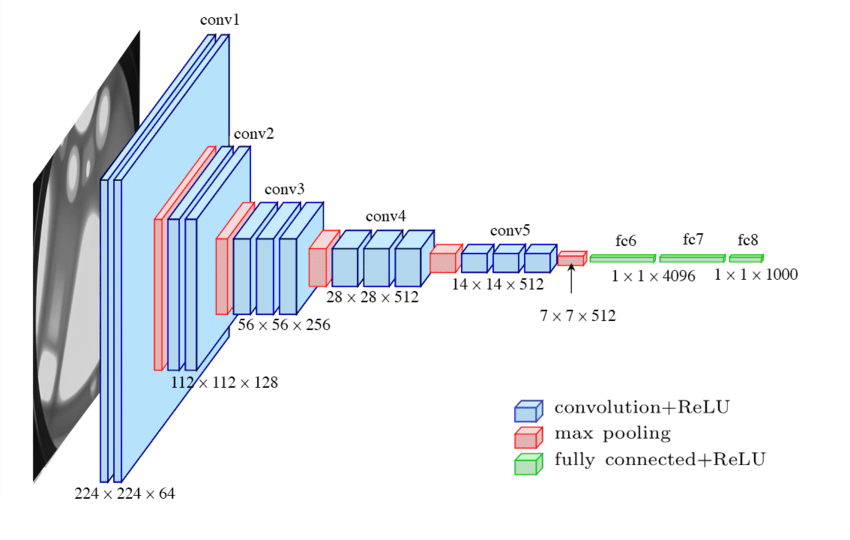
\includegraphics[width=0.95\textwidth]{images/cnn_1.png}
    \caption{CNN architecture of VGG16 \href{https://www.researchgate.net/figure/Fig-A1-The-standard-VGG-16-network-architecture-as-proposed-in-32-Note-that-only_fig3_322512435}{(\underline{source})}}
    \label{fig:cnn_1}
\end{figure}

\subsection{Layers used to build CNN}

\subsubsection{Convolution layer}
The convolution layer is the core building block of the CNN. It carries the main portion of the network’s computational load.

This layer performs a dot product between two matrices, where one matrix is the set of learnable parameters otherwise known as a \textit{kernel} -used to be named $W$ in ANN-, and the other matrix is the restricted portion of the receptive field. The kernel is spatially smaller than an image but is more in-depth. 

If we have an input of size $W \times W \times D$ and $D_{out}$ number of kernels with a spatial size of $F$ with stride $S$ and amount of padding $P$, then the size of output volume $W_{out}\times W_{out}\times D_{out}$ can be determined by the following formula:

\begin{equation} \label{eq:Formula for Convolution Layer}
    W_{out} = \frac{W - F + 2P}{S} + 1
\end{equation}
\myequations{Formula for Convolution Layer}

More visualized example in figure \ref{fig:cnn_2}:

\begin{figure}[h!]
    \centering
    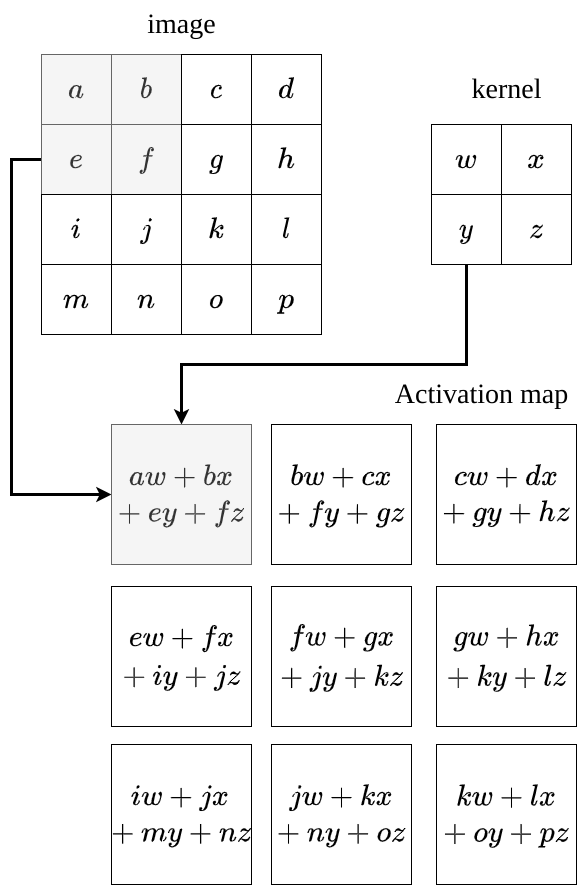
\includegraphics[width=0.8\textwidth]{images/cnn_2.png}
    \caption{Convolution operation}
    \label{fig:cnn_2}
\end{figure}


\subsubsection{Pooling layer}
The pooling layer replaces the output of the network at certain locations by deriving a summary statistic of the nearby outputs. This helps in reducing the spatial size of the representation, which decreases the required amount of computation and weights. The pooling operation is processed on every slice of the representation individually.
There are several pooling functions such as the average of the rectangular neighborhood, L2 norm of the rectangular neighborhood, and a weighted average based on the distance from the central pixel. However, the most popular process is max pooling, which reports the maximum output from the neighborhood.

If we have an activation map of size $W \times W \times D$, a pooling kernel of spatial size $F$, and stride $S$, then the size of output volume $W_{out} \times W_{out} \times D$ can be determined by the following formula:

\begin{equation} \label{eq:Formula for Pooling Layer}
    W_{out} = \frac{W - F}{S} + 1
\end{equation}
\myequations{Formula for Pooling Layer}

More visualized example in figure \ref{fig:cnn_3}:

\begin{figure}[h!]
    \centering
    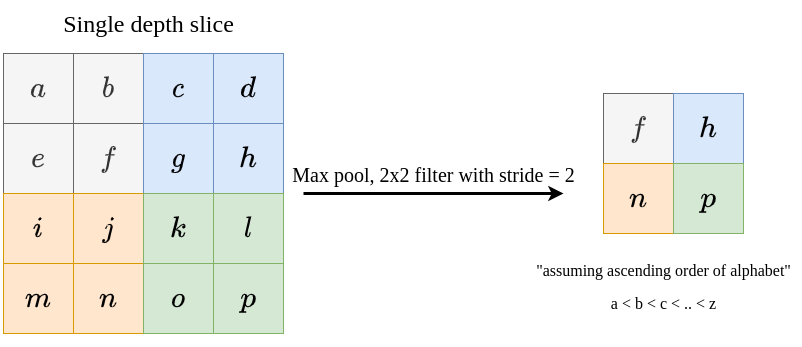
\includegraphics[width=0.8\textwidth]{images/cnn_3.png}
    \caption{Pooling operation}
    \label{fig:cnn_3}
\end{figure}

\subsection{Use case: VGG16 architecture}
As previously seen in figure \ref{fig:cnn_1}, a visualized architecture of VGG16 \cite{vgg}, let us discuss its layers in details.

The input to $cov1$ layer is of fixed size $224 \times 224$ RGB image. The image is passed through a stack of convolutional layers, where the filters (kernels) were used with a very small receptive field: $3 \times 3$. The convolution stride $S$ is fixed to 1 pixel; the spatial padding of $P$ convolutional layer input is such that the spatial resolution is preserved after convolution, i.e. the padding is 1-pixel for $3 \times 3$ convolutional layers. Spatial pooling is carried out by five max-pooling layers, which follow some of the convolutional layers (not all the convolutional layers are followed by max-pooling). Max-pooling is performed over a $2 \times 2$ pixel window, with stride $S = 2$.

Three Fully-Connected (FC) layers follow a stack of convolutional layers: the first two have $4096$ channels each, the third performs 1000-way ILSVRC classification and thus contains 1000 channels (one for each class). The final layer is the softmax layer. The configuration of the fully connected layers is the same in all networks. All hidden layers are equipped with the rectification (ReLU) non-linearity. 
\newpage




\section{Sequence Models}
\label{Sequence Models}
Recurrent neural network (RNN) is a class of artificial neural network, where connections between neurons form a directed graph along a temporal sequence. RNN are able to remember/memorize precise patterns about the input they received, making them more efficient when dealing with \emph{sequential} data such as speech or text.

In our two cases using sequence models we extracted features from \emph{text} to predict meaningful characteristics, that's why we're discussing sequence models with text inputs. Before delving into architectures and techniques, let us define some terminologies needed in this section.

\textbf{Tokenization:} In order to prepare our training corpus, we need to pick the most common and meaningful words that exist, beside pre-processing, tokenization is applied to split the each example of the corpus, count frequencies of each word, and pick the most frequent $N$ ones, $N$ could be in terms of hundreds of thousands or more.

\textbf{Vocabulary}: It's the set of unique words the model is handling, usually they are the set of the most frequent words presented in the whole dataset, see figure \ref{fig:vocabulary}.

\textbf{Encoding}: Words themselves are meaningless to our machines; so an encoding technique is applied to uniquely identify each word with a digit or a vector of digits. Two major techniques are used:
\begin{itemize}
    \item One-hot encoding
    \item Label encoding, similar to tokenization.
\end{itemize}
One-hot encoding replaces each word with a sparse vector composes of all zeros except for the index where the word is located at the vocabulary set, see figure \ref{fig:one-hot encoding}.
Label encoding replaces each word with the index of its location at the vocabulary set, see figure \ref{fig:label encoding}.

\begin{figure}[h!]
    % \centering
    \begin{subfigure}[b]{0.3\textwidth}
    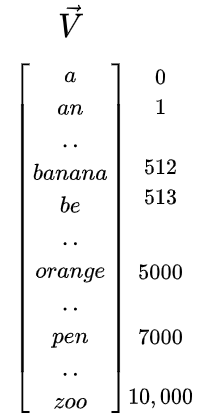
\includegraphics[width=3cm,height=5cm]{images/v.png}
    \caption{Vocabulary V}
    \label{fig:vocabulary}
    \end{subfigure}
    \hfill
    \begin{subfigure}[b]{0.3\textwidth}
        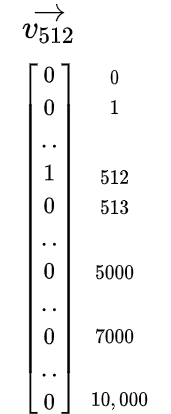
\includegraphics[width=3cm,height=5cm]{images/v_2.png}
        \caption{One-hot encoding}
        \label{fig:one-hot encoding}
    \end{subfigure}
    \hfill
    \begin{subfigure}[b]{0.3\textwidth}
        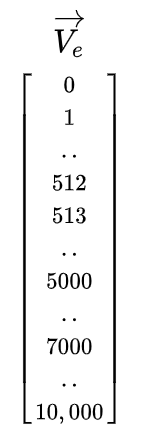
\includegraphics[width=2.5cm,height=5cm]{images/v_3.png}
        \caption{Label encoding}
        \label{fig:label encoding}
    \end{subfigure}
    \caption{Encoding vocabulary}
\end{figure}

\textbf{Dimensions:} Let us define $T_x$ as the length of input vector $X$, where $X[0]$ is the first word in the text input and $X[T_x]$ is the last one, both encoded using one of the previous techniques, similarly for the output vector $y$, where $y[0]$ is the results from feeding the first word to the network and $y[T_y]$ is the result due to the last input word.





\subsection{Architecture} 
Now that we are familiar with sequence models' notations, let's discuss different models' architectures \cite{rnn_models}, we upgraded from ANN to RNN; because of two reasons: one is that inputs and outputs can be different in lengths in different examples, second is ANN does not share features learned across different positions of text.

Different architectures were proposed with various features and characteristics:
\begin{itemize}
    \item Simple RNN
    \item Bidirectional RNN
    \item Long short-term memory (LSTM)
    \item Gated recurrent unit (GRU)
\end{itemize}

\subsubsection{Simple RNN}

\begin{figure}[h]
    \centering
    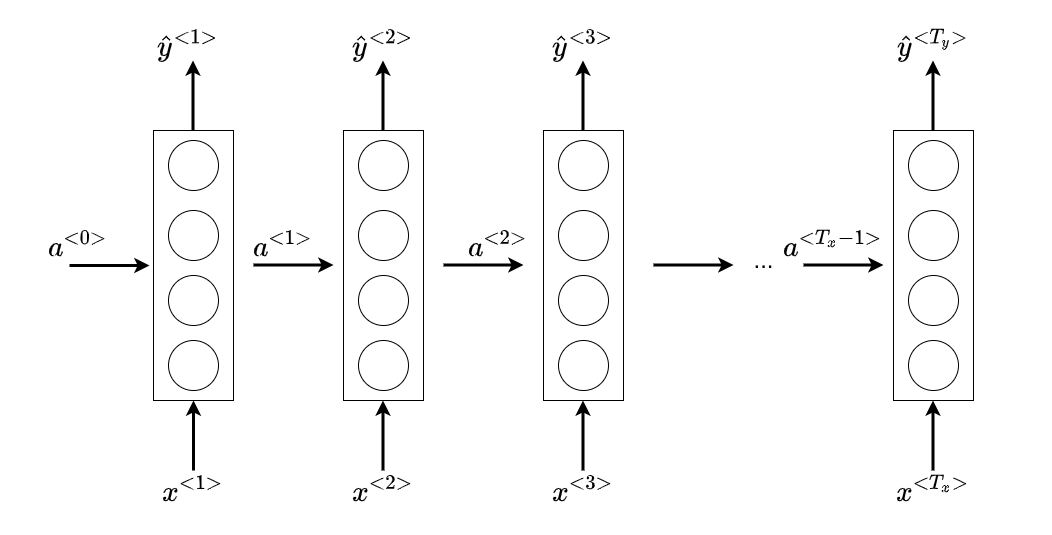
\includegraphics[width=0.9\textwidth]{images/rnn_1.png}
    \caption{Simple unfolded RNN architecture}
    \label{fig:simple_rnn}
\end{figure}
As we can see in figure \ref{fig:simple_rnn} simple RNN models are just repeated ANN models, where information of previous steps are fed to the next one. Each rectangular represents a copy of a chunk of ANN, could be a simple feed-forward ANN, or a more complex one. This chain-like nature reveals that recurrent neural networks are intimately related to sequences and lists. They’re the natural architecture of neural network to use for such data.

Forward propagation in this network works as follows:

\begin{equation} \label{eq:simple_rnn}
\begin{split}
    a^{<t>} &= f_1 \left( W_{aa} a^{<t-1>} +  W_{ax} x^{<t>} \right) \\
    \hat{y}^{<t>} &= f_2 \left( W_{ya} a^{<t>} \right)
\end{split}
\end{equation}
\myequations{Simple RNN forward propagation}

Notice that $f_1$ and $f_2$ could be the same activation functions \ref{sec:activation_function}, but usually $f_1$ is chosen to be \emph{Sigmoid or Tanh}, while $f_2$ to be \emph{ReLU or Softmax}. Also, we used three \textbf{different} weight matrices, $W_{ax}$ is what we used to see back in ANN, but $W_{aa}\; and \;W_{ya}$ are newly defined.

\subsubsection{Long short-term memory (LSTM)}

The problem with RNN is the \emph{long-term dependency}, RNNs are very efficient when it comes to predicting words within a narrow sequence, like predicting the word \textit{"sky"} in this sequence "clouds are in the ...". But, when it comes to predicting text which its background information is captured way before in the context, RNNs seems to fail miserably. The problem was explored in depth by \emph{Hochreiter (1991) [German]} \cite{rnn_long_term_problem_1} and \emph{Bengio, et al. (1994)}, who found some pretty fundamental reasons why it might be difficult.\newline


LSTM figure \ref{fig:lstm} enables the network to remember inputs over a long period of time. LSTM has 3 gates: (input- forget- output) gates:
\begin{itemize}
  \item Input gate: determines whether or not to let the new input in.
  \item Forget gate: deletes the data stored; because they're not important.
  \item Output gate: impact the output at the current timestamp.
\end{itemize} 

\begin{figure}[h]
    \centering
    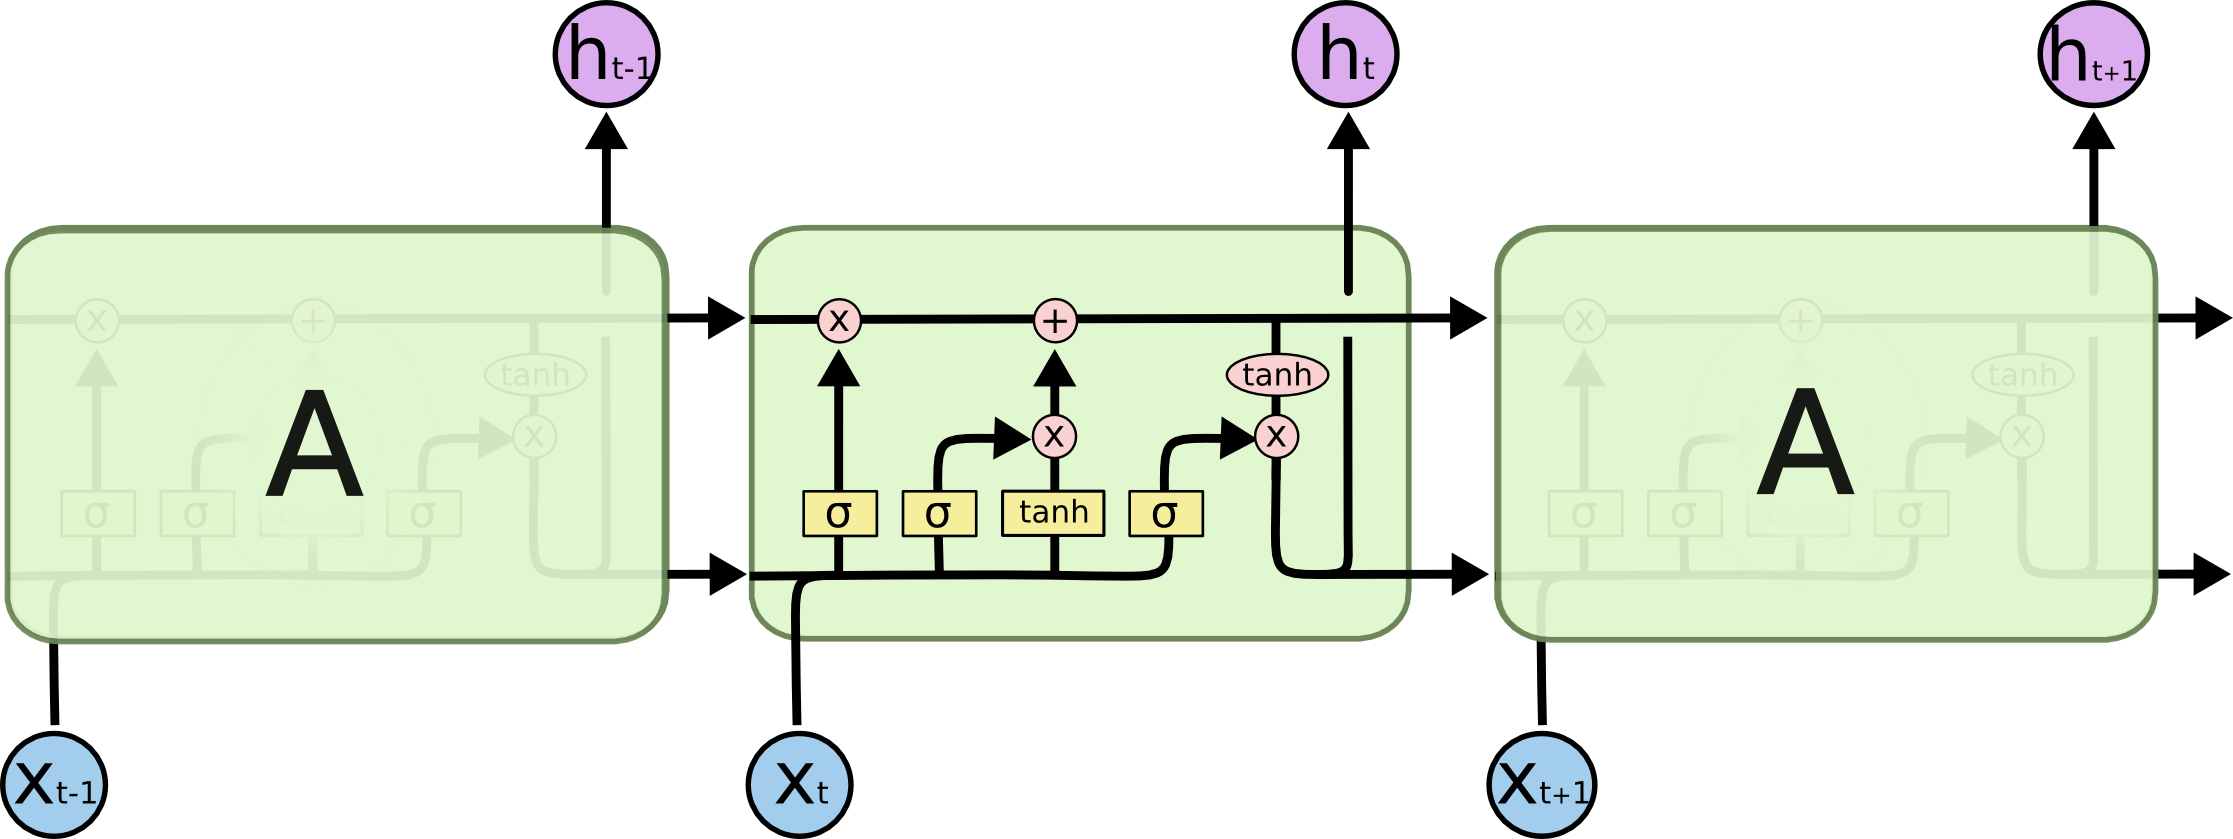
\includegraphics[width=0.9\textwidth]{images/lstm.png}
    \caption{LSTM architecture \href{http://colah.github.io/posts/2015-08-Understanding-LSTMs/}{(\underline{source})}}
    \label{fig:lstm}
\end{figure}


\subsection{Word embedding}
\label{word_embedding}
Word embeddings is a technique used for identifying similarities between words in a corpus by using ANN model to predict the co-occurrence of words within a small chunk of text. Each word is represented by a vector. Word embeddings gained fame in the world of automated text analysis when it was demonstrated that they could be used to identify analogies \cite{Mikolov}.

\textbf{The context window} \\
Word embeddings are created by identifying the words that occur within a “Context Window”. Figure \ref{fig:context_window} illustrates context windows of varied length for a single sentence. The context window is defined by a string of words before and after a focal or “center” word that will be used to train a word embedding model. Each center word and context words can be represented as a vector of numbers that describe the presence or absence of unique words within a dataset, which is perhaps why word embedding models are often described as “word vector” models, or “word2vec” models.

\begin{figure}[h]
    \centering
    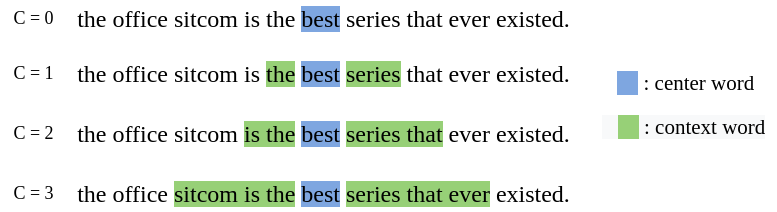
\includegraphics[width=0.9\textwidth]{images/context_window.png}
    \caption{Different sizes of context window}
    \label{fig:context_window}
\end{figure}


\textbf{Embedding matrix}\\
This is how word embeddings are presented, a matrix $\underset{M\times V}{\mathrm{E}}$, where $M$ is the embedding size usually around 200~300, and $V$ is the vocabulary size, usually in order of hundreds of thousands. Each vector is representing a word vector in the vocabulary.



\subsubsection{Word2Vec}
\label{sec:word2vec}
So far so good, but how do we get these embeddings' vectors (embedding matrix)? 
Various mathematical approaches exist for this kind of problem, \emph{count-based methods}, \emph{positive point-wise mutual information}, or \emph{latent semantic analysis}, more on this \href{https://lena-voita.github.io/nlp_course/word_embeddings.html}{(here)}.

Word2Vec is a prediction-based method, an artificial neural network of 2 layers used to learn the context of words. 
Either by predicting the \textit{center} word given the \textit{target} words (CBOW), or predicting \textit{target} words given the \textit{center} word (skip-gram).

Such models could be trained using \emph{Naive Bayes models}, due to the conditional probability nature of the problem, however we are discussing implementing such models using ANN.

Word2vec model takes a large corpus of text dividing them into \textit{center} and \textit{targets}. The system trains them for a number of epochs, aspiring that similar words -in meaning- will have closer values -in word vectors-. Two major types of models exist for this technique, see figure \ref{fig:word2vec_1}:

\begin{itemize}
  \item Continuous Bag-of-Word (CBOW) model
  \item Skip-gram model
\end{itemize}

\begin{figure}[h]
    \centering
    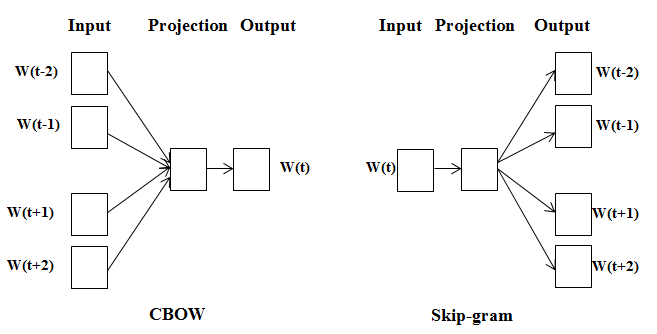
\includegraphics[width=0.9\textwidth]{images/CBOW-and-Skip-gram-models-architecture-1.png}
    \caption{CBOW and Skip-gram models \href{https://www.researchgate.net/profile/Nailah-Al-Madi/publication/319954363/figure/fig1/AS:552189871353858@1508663732919/CBOW-and-Skip-gram-models-architecture-1.png}{(\underline{source})}}
    \label{fig:word2vec_1}
\end{figure}

\textbf{Continuous Bag-of-Word (CBOW) model: }Predicts words (e.g. “mat”) from context words(e.g. “The cat sits on the ...”), it tends to be useful for smaller datasets. \newline

\textbf{Skip-gram: }The inverse of (CBOW) \cite{skip_gram}, it predicts \textit{target} words from \textit{center}, it tends to be useful for larger datasets. \newline




% \subsection{Bidirectional Encoder Representation from Transformer (BERT) Model}
% It’s a pre-trained model designed to be fine tuned with just small additional output to create state of the art wide range or NLP tasks, it’s a very huge model trained on a huge text corpus from both left and right side so it builds a deeper understanding of how the language works.


\subsubsection{Cosine similarity}
\label{cosine}
Cosine similarity is one of the methods to estimate the quality of the learned embeddings. There are several word similarity benchmarks (test sets). They consist of word pairs with a similarity score according to human judgments. The quality of embeddings is estimated as the correlation between the two similarity scores (from model and from humans). 

Equation goes as follows:

% \begin{center}
%     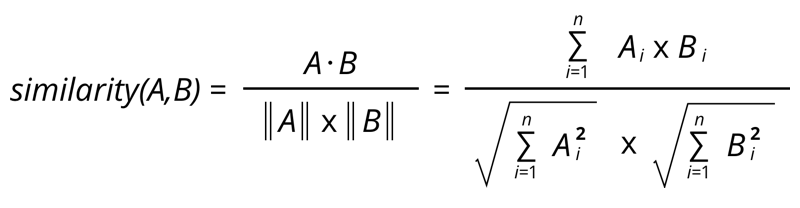
\includegraphics[width=10cm,height=3cm]{images/cosine-similarity.png}
%     % \caption{ReLU activation function }
% \end{center}

\begin{equation} 
\label{eq:cosine_similarity}
   similarity(\Vec{A},\Vec{B}) = \frac{\Vec{A} . \Vec{B}}
   {\Vert{\Vec{A}}\Vert \times \Vert \Vec{B} \Vert }
\end{equation}
\myequations{Cosine similarity}







\subsubsection{Term frequency–inverse document frequency (TF-IDF)}
\label{tfidf}
Although this might seem to be an unrelated topic for sequence models, but we used TF-IDF in evaluating the word2vec model we trained, as we will see in the following chapter.

TF-IDF is a  It is a statistical technique that quantifies the importance of a word in a document based on how often it appears in that document and a given collection of documents (corpus). The intuition for this measure is : If a word occurs frequently in a document, then it should be more important and relevant than other words that appear fewer times and we should give that word a high score (TF). But if a word appears many times in a document but also in too many other documents, it’s probably not a relevant and meaningful word, therefore we should assign a lower score to that word (IDF).

Formula goes as follows:


\begin{equation}
\begin{split}
tf(t,d) &=  \frac{f_{t,d}}{\sum_{t'\in d}f_{t',d}}\\ 
ifd(t,D) &= \log{\frac{N}{1+|d \in D: t \in d|} }\\
tf-idf(i,d) &= tf(i,d) \times idf(i)
\end{split}
\end{equation}
\myequations{TF-IDF}

Where:
\begin{itemize}
    \item N: Number of documents
    \item t: a certain term
    \item d: a certain document
    \item D: all documents
    \item $f_{t,d}$ : is the number of occurrences of $t$ in $d$
\end{itemize}


\section{Transfer Learning}
\label{Transfer Learning}
Transfer learning is a machine learning technique where a model trained on one task is re-purposed on a second related task.

How does it work? In computer vision, for example, artificial neural networks usually try to detect edges in the earlier layers, shapes in the middle layer and some task-specific features in the later layers. In transfer learning, the early and middle layers are used and we only retrain the latter layers. It helps leverage the labeled data of the task it was initially trained on.

In transfer learning, we try to transfer as much knowledge as possible from the previous task the model was trained on to the new task at hand. This knowledge can be in various forms depending on the problem and the data. For example, it could be how models are composed, which allows us to more easily identify novel objects.

Approaches to transfer learning:

\begin{itemize}
    \item \textbf{Training a model to reuse it: }when facing a task A but data is scarce, one way to conquer it is training another model B with similar features having a sufficient amount of data, and use that model as a starting point for task A.
    \item \textbf{Using a pre-trained model: }downloading them or using built-in implemented models on frameworks such as \textit{Keras}, which provides nine pre-trained models that can be used for transfer learning, prediction, feature extraction and fine-tuning. 
    \item \textbf{Feature extraction: }another approach is to use deep learning to discover the best representation of the problem, which means finding the most important features.
\end{itemize}

Most common pre-trained models used for transfer learning that we used in our comparative studies and implementation:

\begin{itemize}
    \item \textbf{BERT (Bidirectional Encoder Representations from Transformers)} is a recent paper published by researchers at Google AI Language \cite{bert}. It has caused a stir in the Machine Learning community by presenting state-of-the-art results in a wide variety of natural language processing tasks, including question answering.
    
    \item \textbf{VGG-16} is a convolution neural net (CNN ) architecture which was used to win ILSVR(Imagenet) competition in 2014 \cite{vgg}. It is considered to be one of the excellent vision model architecture till date.
    
    \item \textbf{gensim-models} \href{https://radimrehurek.com/gensim/}{\textit{gensim}} library has various built-in models for text mining, that are easy to be downloaded and run, trained or tuned for a specific purpose, one of these models is \textbf{word2vec-google-news-300}. We used it for verifying our resume ranker model.
\end{itemize}


\newpage

\section{Rest API}
\label{sec:Rest API}
A REST API (also known as RESTful API) is an application programming interface (API) that follows the rules of REST architectural style and allows for interaction with RESTful web services. REST stands for representational state transfer and was created by computer scientist Roy Fielding \cite{rest}.

An API is a set of definitions and protocols for building and integrating application software. It’s sometimes referred to as a contract between an information provider and an information user—establishing the content required from the consumer (the call, in our case front-end) and the content required by the producer (the response, in our case back-end). 

An API is a mediator between users and resources or web services they want to acquire. It’s also a way for an organization to share resources and information while maintaining security, control, authentication, and determining who gets access to what resource.

The data in a REST API is usually transferred as a JSON. Requests of a REST API should be independent and don't store user state unlike sessions, and that leads to the ability of sending different requests to different machines that hold the back-end.

There are 4 main operations that we do using the REST API:
\begin{enumerate}
    \item \textbf{GET}: request a resource from the server
    \item \textbf{POST}: store a resource to the server
    \item \textbf{PUT/PATCH}: modify a resource in the server.
    \item \textbf{DELETE}: delete a resource from the server.
\end{enumerate}

\section{CAP Theorem}
\label{sec:cap}
CAP theorem stands for consistency, availability and partition tolerance, and it states that these 3 concepts can't be achieved together, at most you can achieve only 2 of them at the same time.

Consistency means that if you have the data stored as copies on different machines, all the copies should be the same. 
Availability ensures that when the user requests data, he should get it right away.
Partition tolerance is the ability of the system to still function if there is a failure in a portion of the network.

If you want to achieve consistency and availability, you can't achieve partition tolerance, because those 2 can't be achieved at the same time if there is a partial failure in the network. 
If you want to achieve availability and partition tolerance, you can't guarantee consistency, because if the user requests data from a node he will get it, and will not wait until the network failure is fixed, and the data is consistent in that node. 
If you want to achieve consistency and partition tolerance, you can't guarantee availability, because the user will have to wait until the data is transferred and consistent.

\section{Load Balancing}
\label{sec:Load}
Load balancing is distributing the work across multiple machines and is used when one machine can't handle all the requests it receives.

It may be simple as round robin (the requests are sent to machines in their order, cycling back when reaching the last machine), but this can lead overwhelming a certain machine with heavy requests, suppose that we have only 2 machines, and all the odd requests are simple, and all the even requests are heavy, so the first machine doesn't have a lot of work to do and is almost idle, but the second machine is almost busy all the time. 
To overcome this problem, load balancing can be implemented such that it waits for a machine to be idle, then it sends the next request to it.

There are other algorithms to perform load balancing, such as weighted round robin, hashing which assigns the request based on its hash value, and least connection which assigns the request to the node that has the lowest number of connections.

\newpage
\section{Comparative Study of Previous Work}
\label{sec:comparitive}
In this section we show some of the most important works that we got inspired from and challenged during the implementation and evaluation of our agents.\\
\begin{enumerate}
    \item \textbf{Deepface}: is a lightweight face recognition and facial attribute analysis (age, gender, emotion and race) framework for python. It is a hybrid face recognition framework wrapping state-of-the-art models: VGG-Face, Google FaceNet, OpenFace, Facebook DeepFace, DeepID, ArcFace and Dlib. Those models already reached and passed the human level accuracy. The library is mainly based on Keras and TensorFlow \cite{deepface}.
    
    \item \textbf{Arriaga et al.}: in 2017 they proposed a paper named "Real-time Convolutional Neural Networks for Emotion and Gender Classification" \cite{ariaga} that we implemented for the purpose of emotion detection based on images extracted from video.
    
    \item \textbf{Who Am I? Personality Detection Based on Deep Learning for Texts}: they combined embedding layer and LSTM with a three CNN layers. Validation accuracy did not exceed the benchmark set for the problem of personality detection based on text \cite{who am i}.
    
    \item \textbf{Yash et al.}: they provided a thorough survey into the problem of personality detection based on text, training on two different datasets; one for OCEAN characteristic and the other for psycho-linguistic characteristic, combined them and tried each one separately, with different models for features extraction, and for classification (ANN and SVM). Results did not improve much, they also maintained a range of $60\%$ validation accuracy \cite{yash}.
    
    \item \textbf{Hans et al.}: they were able to achieve $86\%$ validation accuracy in the problem of personality prediction based on text; because they were able to reach a very large dataset, enabling them to capture more powerful features \cite{hans}.
    
    \item \textbf{Amirmohammad et al.}: we used this paper as a reference while implementing the personality analysis model. They used a similar approach for feature extraction (using BERT), but combined it with SVM classifier instead of ANN \cite{yash_2}.
    
    
\end{enumerate}

\newpage

\section{Implemented Approach}
\label{sec:implemented}
We implemented three different AI models, one for each task, emotion detection, personality analysis and resume ranking. In addition to this we designed our system to be in a distributed form, balancing work loads among workers.\\
\begin{enumerate}
    \item\textbf{Emotion detection}\\
    We implemented the CNN architecture proposed in \cite{ariaga}. Initially we did not have any intuition how we can modify the current architecture, and later on settled on maintaining the current architecture as we compared it with VGG16, and found that our model behaves faster, with higher accuracy, and less memory space occupation (see \ref{sec:emotion_testing} for more).
    
    \item\textbf{Personality analysis}\\
    From the start we knew that sequence models will be needed for the purpose of this problem, that is why we followed several recently published papers (mentioned previously), and finally settled on implementing \cite{yash_2}; not only because of the different architecture they used but also because the results are humanly meaningful.
    
    \item \textbf{Resume ranker}\\
    We did not follow any paper or even find an acceptable related work for this problem. However, based on previous knowledge in the field of sequence models we adopted the architecture of word2vec \ref{sec:word2vec} to conquer the problem; training a reasonable embedding matrix \ref{word_embedding} using a large set of resumes in different fields, and then used two different ranking techniques: cosine similarity and TF-IDF, generally we used \href{https://radimrehurek.com/gensim/}{\textit{gensim}} library for the task of training word2vec models.
    
    \item \textbf{Distributed system}\\
    As you can expect by now, running all of these models in production time will take much time; that's why the back-end side of the application is implemented using \href{https://www.rabbitmq.com/}{\textit{RabbitMQ}} library, allowing us to distribute the loading among several nodes (machines) and maintain a fault tolerance state of the whole application (more on that later).
    
\end{enumerate}


% Conclude this chapter by this section stating the approach chosen from those reviewed, but more important your justification why you chose this approach along with any modifications added to the approach.
% Notice, you may be implementing several techniques however you must illustrate the general framework for your approach.